%% ceci est un commentaire 
%% il faut toujours commencer par \documentclass[type de papier, taille de texte]{sytle du document}
\documentclass[a4paper,10pt]{report} %%%% sytle du document : report/book/article


%%%%%%%%%%%%%%%%%%%%%%%%%%%%%%%%%%%%%%%%%%%%%%%%%%%%%%%%%%%%%%%%%%%%%%%%%%%%%%%
%% la suite est une collection des "package" ou des "librararies" pour utiliser des codes spécifiques

%% il vous suffit de les copie-coller quand vous créez un nouveau document TeX (ou bien en ajouter plus si besoin).
\usepackage[utf8]{inputenc} %% pour les accents en français
\usepackage[frenchb]{babel} %% pour un format français
\usepackage{graphicx} %% pour afficher des graphiques
\usepackage{amsmath} %% pour écrire des symboles (maths), des équations, etc.
\usepackage{amssymb}
\usepackage{color}
\usepackage{bm} %% pour lister des citations/la biblio
\usepackage{hyperref} %% pour inserer des liens internet
\usepackage{cleveref} %% pour faire des références uax équations, tableaux, etc.
%\usepackage{setspace} %% pour changer l'espace entre les lignes
%\linespread{1.6} %% pour changer l'espace entre les lignes












%%%%%%%%%%%%%%%%%%%%%%%%%%%%%%%%%%%%%%%%%%%%%%%%%%%%%%%%%%%%%%%%%%%%%%%%%%%%%%%
\title{--------TITRE--------} %% choissez un titre approprié à votre sujet
\author{par\\DUPONT, Béatrix\\ MARTIN, Asterix\\pour le DM de l'UE Outils pour la Mécanique - Maths (M1)} %% utilisez \\ pour une novuelle ligne
\date{fait le 05 septembre 2016} %% pour afficher la date actuelle commenter cette ligne














%%%%%%%%%%%%%%%%%%%%%%%%%%%%%%%%%%%%%%%%%%%%%%%%%%%%%%%%%%%%%%%%%%%%%%%%%%%%%%%
%% TOUT ce qui va dans votre rapport doit être entre \begin{document} & \end{document}
\begin{document}
\selectlanguage{french} %% format français
\maketitle %% pour afficher le titre
\tableofcontents %% pour afficher/compiler le sommaire automatiquement
\listoffigures %% pour lister les figures













%%%%%%%%%%%%%%%%%%%%%%%%%%%%%%%%%%%%%%%%%%%%%%%%%%%%%%%%%%%%%%%%%%%%%%%%%%%%%%%
\chapter{Consignes Générales} %% pour commencer un chapitre
Votre rapport/compte-rendu doit-être rendu en format PDF et il devrait-être écrit en LaTeX.
















%%%%%%%%%%%%%%%%%%%%%%%%%%%%%%%%%%%%%%%%%%%%%%%%%%%%%%%%%%%%%%%%%%%%%%%%%%%%%%%
\section{Avant Propos} %% pour commencer une section
\label{sec:AP} %% une libelle qu'on peut utiliser pour référer à cette section
Vous pouvez utiliser les postes de travail dans les salles informatiques duu département pour écrire en \textbf{LaTex} et utiliser \textbf{TexMaker} (un environnent pour travailler avec \textbf{LaTeX}). Vous pouvez aussi les installer sur votre ordinateur.
\begin{itemize} %% une liste simple
\renewcommand{\labelitemi}{$\circ$}
	\item Pour une installation en \textbf{WINDOWS} : \href{http://www.howtotex.com/howto/installing-latex-on-windows/}{cliquez ici}.
	
	\item Pour une installation en \textbf{MAC OS X} : \href{http://www.howtotex.com/howto/installing-latex-on-mac-os-x/}{cliquez ici}.
	
	\item Pour une installation en \textbf{LINUX} : \href{http://www.howtotex.com/howto/installing-latex-on-mac-os-x/}{cliquez ici}.
\end{itemize}














%%%%%%%%%%%%%%%%%%%%%%%%%%%%%%%%%%%%%%%%%%%%%%%%%%%%%%%%%%%%%%%%%%%%%%%%%%%%%%%
\section{Contenu} %% pour commencer une section
\label{sec:contenu}
Dans la manière générale, il doit contenir :
\begin{enumerate} %% une liste numérotée
	\item Sommaire (Table of Contents).
	\item Liste des figures (Table of Figures)
	\item Liste des symboles (Table of Symbols)
    \item Chapitre $1$ : Introduction \& Modélisation par Éléments Finis (avec des sections qui expliquent le problème physique, la formulation faible, la forme d'approximation/interpolation, les expressions des matrices A \& B --avec démonstrations).
    \item Chapitre $2$ : Résolution numérique (avec des sections qui donnent l'algorithme, les commentaires sur la programmation/program, validation du code).    
    \item Chapitre $3$ : Résultats \& Conclusions (avec des sections qui indiquent les résultats obtenus/demandés $+$ des commentaires critiques, conclusion finale qui synthétise tous les résultats principaux obtenus, et finalement, perspectives de vos travaux).
    \item La liste de bibliographie.
    \item Les annexes (codes python/matlab/etc.)
\end{enumerate} 














%%%%%%%%%%%%%%%%%%%%%%%%%%%%%%%%%%%%%%%%%%%%%%%%%%%%%%%%%%%%%%%%%%%%%%%%%%%%%%%
\chapter{Quelques Syntax en LaTeX} %% pour commencer un chapitre
Pour un simple guide (le plus simple que je connais !) pour LaTex \href{http://www.howtotex.com/download/FiveMinuteGuideToLaTeX.pdf}{cliquez ici}.













%%%%%%%%%%%%%%%%%%%%%%%%%%%%%%%%%%%%%%%%%%%%%%%%%%%%%%%%%%%%%%%%%%%%%%%%%%%%%%%
\section{Equations}
\label{sec:eqn}

\subsection{Symboles mathématiques}
Une liste décrivant quasi-totalité des symboles classiques se trouve dans le wiki suivant : \href{https://en.wikibooks.org/wiki/LaTeX/Mathematics}{WikiBooks--LaTeX/Mathematics}.

\subsection{Comment faire}
D'une façon simple et efficace, vous pouvez inclure les expressions mathématiques dans le text en les mettant entre \$ et \$; par exemple, $\alpha^2 + \beta^2 = 1$. Vous pouvez aussi écrire des équations/expressions mathématiques en déhors du paragraphe en les mettant entre \$\$ et \$\$; par exemple, $$\alpha^2 + \beta^2 = 1.$$
Toute fois, si vous souhaitez les numéroter, vous pouvez utiliser
	\begin{equation}
		E = \frac{1}{2} m v^2
		\label{eq:example1}%%libelle à utiliser pour citer cette équation dans le texte
	\end{equation}
Une libelle ($\backslash$label\{\}) permet de faire des références aux équations précédentes ou de les citer, par exemple, l'énergie cinétique d'une particule se calcule via éqn (\ref{eq:example1}).













%%%%%%%%%%%%%%%%%%%%%%%%%%%%%%%%%%%%%%%%%%%%%%%%%%%%%%%%%%%%%%%%%%%%%%%%%%%%%%%
\section{Figures \& Tableaux}
\label{sec:FigTables}
Il faut que vos graphiques soient déjà stockés dans une location précises sur votre ordinateur. Par exemple, le plus simple est de les stocker dans le même dossier que votre ficher TeX mais une bonne pratique est de les garder dans un  dossier nommé FIG dans le même dossier que votre fichier TeX. Ensuite utilisez le code suivant :\\
%%%%%%%%%%%%%%%%%%%%%%%%%%%%%%%%%%%%%%%%%%%%%%%%%%%%%%%%%%%%%%%%%%%%%%%%%%%%%%%
$\backslash$begin\{figure\}[h]\\
$\backslash$begin\{center\}\\
$\backslash$includegraphics[width=0.35$\backslash$textwidth]\{FIG/FileName.png\}\\
$\backslash$end\{center\}\\
$\backslash$caption\{Titre du graphique et une explication biève\}\\
$\backslash$label\{fig:sonLibelle\}\\
$\backslash$end\{figure\}\\

Voici un exemple,
\begin{figure}[h]
%% [h] implique que le graphique sera placé ici (et pas en haut ou en bas du document)
\begin{center}
%% pour centré l'image
	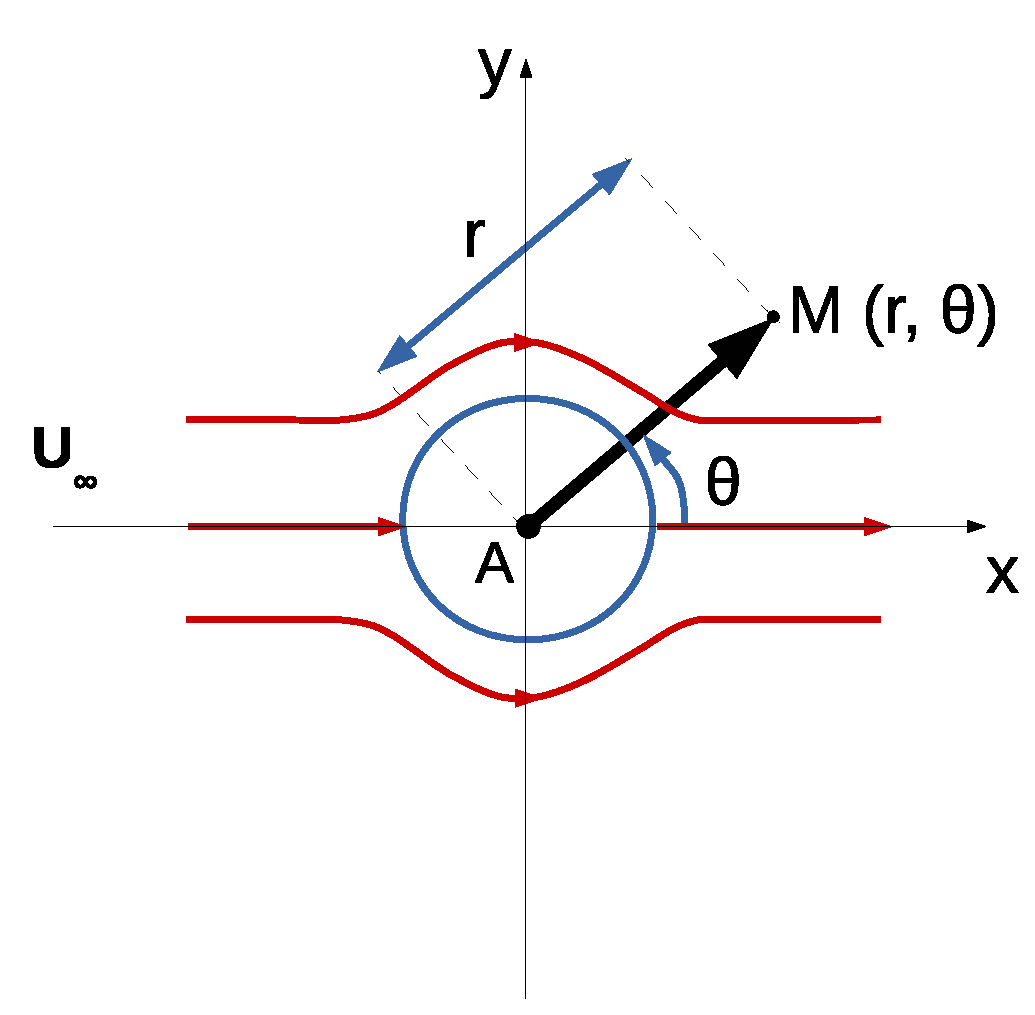
\includegraphics[width=0.5\textwidth]{FIG/fiGGs_polar.eps}
	%% 0.35 fois le largeur du document (\textwidth)
\end{center}
\caption{Écoulement autour d'un cylindre $2D$ en coordonnées cartésiennes/polaires.}
\label{fig:figureCoorPol}
\end{figure}














%%%%%%%%%%%%%%%%%%%%%%%%%%%%%%%%%%%%%%%%%%%%%%%%%%%%%%%%%%%%%%%%%%%%%%%%%%%%%%%
\section{Citations}
\label{sec:Biblio}
Il faut creer un fichier BibTeX (par exemple, MonBiblio.bib) et l'appeler (avant la fin du document; avant $\backslash$end\{document\}) avec $\backslash$bibliography\{MonBiblio.bib\}. Vous pouvez ajouter
$\backslash$bibliographystyle\{unsrtnat\} pour trier les citations en ordre de citation.

Par exemple, avec le fichier MonBiblio.bib, je cite quand j'emprunte une formule d'un ouvrage \cite{Auteur1_Livre} ou bien des citations d'un article \cite{Auteur_ArticleSci}. Quoi que ça soit, vous devez impérativement citer vos sources pour le compte-rendu.

ATTENTION : il faudra d'abord compiler BibTex avec succès avant de compiler LaTeX dans TexMaker et ce dernier en plusieurs fois pour que vos références affiche sans points d'interrogations.

\begin{center}
--------------\\
TOUTE FOIS, JE RESTE À VOTRE DISPOSITION POUR VOUS AIDER À PRÉPARER UN MANUSCRIT BIEN ÉCRIT EN LATEX. MAIS JE NE POURRAIS PAS VOUS AIDER POUR L'INSTALLATION DU LOGICIEL MIKETEX ET TEXMAKER.\\
---------------
\end{center}

\bibliography{MonBiblio.bib}
\bibliographystyle{unsrtnat}	
\end{document}
\grid
